\documentclass{article} 
\usepackage{tikz} 
\begin{document} 
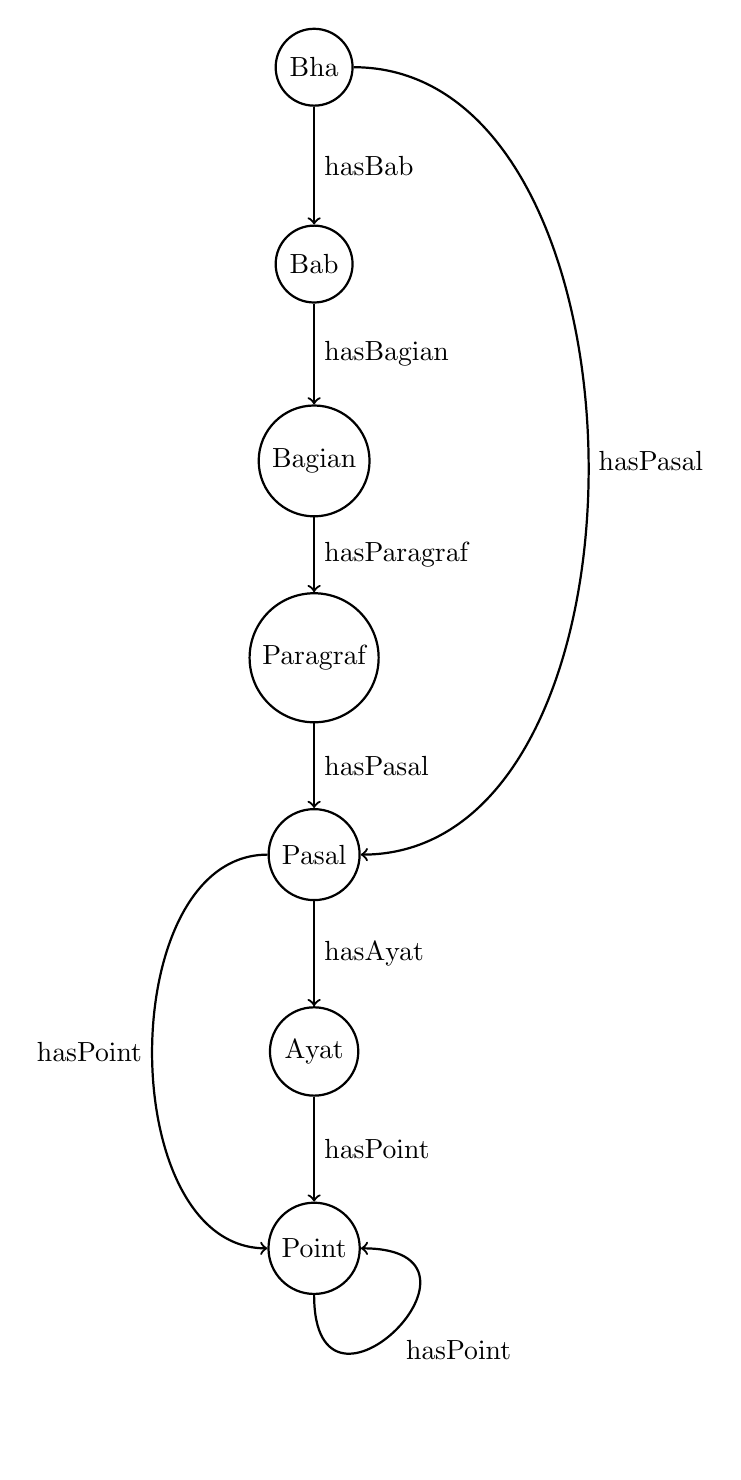
\begin{tikzpicture}[node distance={25mm}, thick, main/.style = {draw, circle}] 
\node[main] (doc) {Bha}; 
\node[main] (bab) [below of=doc] {Bab};
\node[main] (bagian) [below of=bab] {Bagian};
\node[main] (paragraf) [below of=bagian] {Paragraf};
\node[main] (pasal) [below of=paragraf] {Pasal};
\node[main] (ayat) [below of=pasal] {Ayat};
\node[main] (point) [below of=ayat] {Point};
\draw[->] (doc) -- node[midway, right] {hasBab} (bab);
\draw[->] (bab) -- node[midway, right] {hasBagian} (bagian);
\draw[->] (bagian) -- node[midway, right] {hasParagraf} (paragraf);
\draw[->] (paragraf) -- node[midway, right] {hasPasal} (pasal);
\draw[->] (doc) to [in=0, out=0] node[midway, right] {hasPasal} (pasal);
\draw[->] (pasal) -- node[midway, right] {hasAyat} (ayat);
\draw[->] (pasal) to [in=180, out=180] node[midway, left] {hasPoint} (point);
\draw[->] (ayat) -- node[midway, right] {hasPoint} (point);
\draw[->] (point) to [in=0, out=270, looseness=6] node[midway, below right] {hasPoint} (point);
\end{tikzpicture} 
\end{document}